
%(BEGIN_QUESTION)
% Copyright 2008, Tony R. Kuphaldt, released under the Creative Commons Attribution License (v 1.0)
% This means you may do almost anything with this work of mine, so long as you give me proper credit

One of the problems with simple on-off control is that the final control element ``cycles'' frequently.  In real life, this may be a problem because frequent cycling means more wear and a shortened lifespan for the component.

An answer to this problem of frequent cycling is to design the system to have a ``gap'' or a ``band'' of control rather than a single setpoint.  In effect, there are two setpoints: an upper and a lower setpoint.  This is commonly referred to as {\it differential gap control}, or alternatively as {\it on-off control with deadband}.  Shown here is a simple switch-and-relay circuit for a differential gap oven temperature control:

$$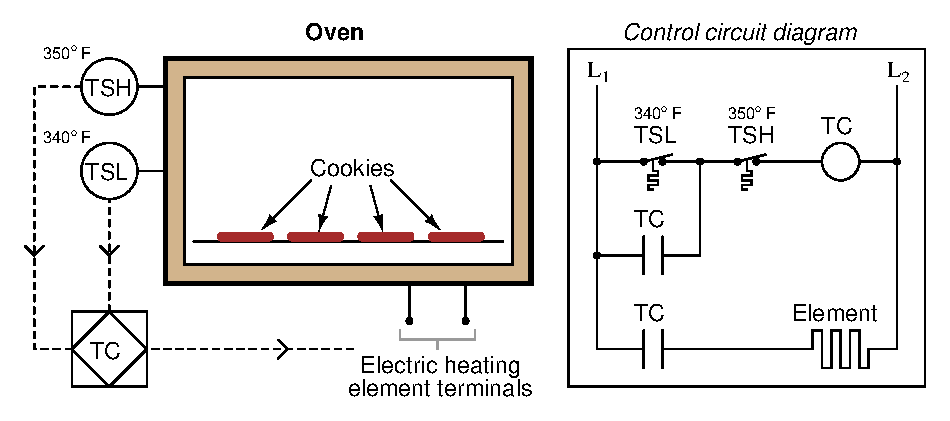
\includegraphics[width=15.5cm]{i01450x01.eps}$$

In the case of this electric oven, differential gap control means the heating element will not turn on until the temperature falls below the lower setpoint, and will not turn off until the temperature rises above the upper setpoint:

$$\includegraphics[width=15.5cm]{i01450x02.eps}$$

Graph this oven's temperature over time as the control system operates, and contrast its behavior against that of a single-point on-off control system.

\underbar{file i01450}
%(END_QUESTION)





%(BEGIN_ANSWER)

$$\includegraphics[width=15.5cm]{i01450x03.eps}$$

%(END_ANSWER)





%(BEGIN_NOTES)

The behavior of a differential gap control system is quite a bit ``looser'' than that of a simple (single-point) on-off control, but at least we do not cycle the final control element nearly as often.

\vskip 20pt \vbox{\hrule \hbox{\strut \vrule{} {\bf Virtual Troubleshooting} \vrule} \hrule}

This question is a good candidate for a ``Virtual Troubleshooting'' exercise.  Presenting the diagram to students, you first imagine in your own mind a particular fault in the system.  Then, you present one or more symptoms of that fault (something noticeable by an operator or other user of the system).  Students then propose various diagnostic tests to perform on this system to identify the nature and location of the fault, as though they were technicians trying to troubleshoot the problem.  Your job is to tell them what the result(s) would be for each of the proposed diagnostic tests, documenting those results where all the students can see.

During and after the exercise, it is good to ask students follow-up questions such as:

\begin{itemize}
\item{} What does the result of the last diagnostic test tell you about the fault?
\item{} Suppose the results of the last diagnostic test were different.  What then would that result tell you about the fault?
\item{} Is the last diagnostic test the best one we could do?
\item{} What would be the ideal order of tests, to diagnose the problem in as few steps as possible?
\end{itemize}

%INDEX% Control, basics: differential gap control (electromechanical relay)
%INDEX% Control, basics: on/off control (with deadband)
%INDEX% Process: cookie baking oven

%(END_NOTES)


